\intro{}


\section{Array}
\subsection{Definizione e idea intuitiva di array}
\defn{Array}{
Un array è una collezione di un numero fisso di elementi, tutti dello stesso tipo, memorizzati in celle di memoria contigue.

}
Dal punto di vista sintattico, la dichiarazione di un array in C++ segue la forma generale:
\begin{codebox}
\begin{lstlisting}
  dataType arrayName[intExp];
\end{lstlisting}
\end{codebox}

dove \inlinecode{dataType} indica il tipo degli elementi, \inlinecode{arrayName} è il nome attribuito all’array e \inlinecode{intExp} è un'espressione costante positiva che specifica il numero di componenti. È importante osservare che la dimensione così indicata rimane fissa per tutta la durata di vita dell’array: una volta dichiarato, non è possibile aumentare o diminuire il numero di elementi senza creare una nuova struttura e copiarvi i dati.



\subsection{ Limiti degli array e motivazione per strutture più astratte}

Gli array forniscono un meccanismo essenziale per rappresentare sequenze di valori omogenei in memoria contigua, con accesso diretto tramite indice. Tuttavia, proprio le caratteristiche che li rendono semplici ed efficienti ne evidenziano anche alcuni limiti strutturali, che diventano rilevanti nella progettazione di programmi complessi.

Un primo limite riguarda la rigidità della dimensione. La lunghezza di un array deve essere nota al momento della dichiarazione e rimane invariata per tutta la vita dell'array.

Ciò obbliga il programmatore a stimare in anticipo il numero massimo di elementi necessari: una scelta troppo prudente porta a spreco di memoria, mentre una stima troppo ottimistica può risultare insufficiente in casi reali d'uso. In altre parole, l’array è un contenitore statico, poco adatto a modellare collezioni la cui cardinalità può variare in modo significativo durante l'esecuzione.

Un secondo limite è legato alla mancanza di informazione incorporata sulla dimensione logica. Quando un array viene passato a una funzione, esso “decade” in un puntatore al suo primo elemento; la funzione riceve quindi solo un indirizzo di memoria, e non ha più accesso diretto alla dimensione dell’array originario. Di conseguenza, è necessario trasmettere esplicitamente un parametro aggiuntivo che rappresenti la lunghezza effettiva della sequenza, con il rischio di introdurre incoerenze tra i dati e le informazioni di supporto, oppure di incorrere in accessi fuori dai limiti qualora tali parametri non vengano gestiti con attenzione.


Inoltre, gli array non mettono a disposizione operazioni ad alto livello per la gestione dinamica dei dati. Non esistono primitive del linguaggio per inserire o rimuovere elementi all'interno della sequenza, per ridimensionare il contenitore o per verificarne automaticamente i limiti; tali operazioni devono essere simulate manualmente, spostando gli elementi e gestendo direttamente la memoria sottostante. Questa mancanza di astrazione aumenta la complessità del codice applicativo e rende più probabile l'introduzione di errori legati alla gestione della memoria, agli indici e alla coerenza dei dati.







Inoltre, gli array non mettono a disposizione operazioni ad alto livello per la gestione dinamica dei dati. Non esistono primitive del linguaggio per inserire o rimuovere elementi all’interno della sequenza, per ridimensionare il contenitore o per verificarne automaticamente i limiti; tali operazioni devono essere simulate manualmente, spostando gli elementi e gestendo direttamente la memoria sottostante. Questa mancanza di astrazione aumenta la complessità del codice applicativo e rende più probabile l’introduzione di errori legati alla gestione della memoria, agli indici e alla coerenza dei dati.



















\section{Vector}
\subsection{Idea generale}
\defn{Vector}{
 Un vector è un array dinamico: una sequenza ordinata di elementi omogenei memorizzati in celle di memoria contigue, la cui dimensione può variare durante l'esecuzione del programma. A differenza degli array statici, il \inlinecode{std::vector} integra la gestione automatica della memoria e mette a disposizione operazioni ad alto livello per inserire, rimuovere e accedere agli elementi.
}
 Dal punto di vista pratico , per utilizzare un \inlinecode{std::vector} in C++ la prima operazione necessaria è includere l'header della libreria standard che ne definisce l'interfaccia tramite la direttiva \inlinecode{\#include <vector>}.  




Una dichiarazione tipica è
\inlinecode{std::vector<int> v;}, che crea un vettore di interi vuoto,
la cui dimensione iniziale è 0.
In alternativa, la dichiarazione
\inlinecode{std::vector<int> v(100);}
costruisce un vettore con 100 elementi già presenti,
tutti inizializzati a 0.

Il punto chiave è che la dimensione logica del container
(non il tipo \inlinecode{std::vector<int>} in sé)
non è più una costante fissata staticamente come negli array,
ma uno stato interno dell'oggetto che può cambiare
durante l'esecuzione del programma.

\subsection{Struttura interna}

Dal punto di vista implementativo, \inlinecode{std::vector<T>} è un oggetto
che incapsula tre campi fondamentali:

\begin{itemize}
    \item un \textbf{puntatore} al buffer contiguo in memoria, dove sono
          effettivamente memorizzati gli elementi di tipo \inlinecode{T};
    \item \textbf{size}: un intero che rappresenta il numero di elementi
          attualmente presenti nel vettore;
    \item \textbf{capacity}: un intero che indica quanta memoria è stata
          riservata, ovvero quanti elementi possono essere contenuti prima
          che sia necessaria una riallocazione.
\end{itemize}

In generale vale sempre $\text{size} \leq \text{capacity}$:
quando si inserisce un elemento con \inlinecode{push\_back} e la size
raggiunge la capacity, il vector alloca automaticamente un nuovo buffer
più grande (tipicamente raddoppia la capacity), copia gli elementi

\subsection{Metodi principali}

Su questo oggetto \`e possibile chiamare i seguenti metodi:

\begin{itemize}
    \item \inlinecode{v.size()}: restituisce il numero di elementi logici
          attualmente contenuti nel vettore.

    \item \inlinecode{v.at(i)}: restituisce un riferimento all'elemento
          in posizione \inlinecode{i}, con controllo dei limiti.
          Se \inlinecode{i} \`e fuori dall'intervallo valido,
          lancia un'eccezione di tipo \inlinecode{std::out\_of\_range},
          causando un errore controllato anzich\`e un comportamento
          indefinito come con l'operatore \inlinecode{[]}.

    \item \inlinecode{v.resize(n)}: modifica la dimensione logica del
          vettore portandola a \inlinecode{n}. Se \inlinecode{n} \`e
          maggiore della size attuale, i nuovi elementi vengono
          inizializzati al valore di default del tipo (ad esempio
          \inlinecode{0} per \inlinecode{int}); se \inlinecode{n} \`e
          minore, gli elementi in eccesso vengono rimossi.

    \item \inlinecode{v.push\_back(x)}: aggiunge un nuovo elemento
          in coda al vettore, incrementando la size di 1.
          Se necessario, viene eseguita una riallocazione automatica
          del buffer interno.
\end{itemize}

\subsection{Passaggio dei parametri}



\begin{codeexample}[Passaggio dei parametri]
Un \inlinecode{std::vector} viene tipicamente passato alle funzioni
\textbf{per riferimento} , evitando la copia dell'intero
buffer e permettendo alla funzione di modificare il contenuto originale.



    \begin{codebox}

\begin{lstlisting}
void foo(vector<int>& v) {
    v.at(2) = 0;
}

int main() {
    vector<int> v {1, 2, 3, 4, 5};
    foo(v);
    cout << v.at(2);
    return 0;
}
\end{lstlisting}
\end{codebox}
\end{codeexample}

In questo esempio, \inlinecode{foo} riceve il vettore per riferimento
e modifica l'elemento in posizione 2. La chiamata
\inlinecode{cout<< v.at(2)} nel \inlinecode{main} stamper\`a quindi
\inlinecode{0}, confermando che la modifica ha effetto sull'oggetto
originale e non su una copia.

Il simbolo \inlinecode{\&} nella firma \inlinecode{vector<int>\& v} implica che
\inlinecode{v} \`e un \textbf{riferimento} al vettore originale: all'interno di
\inlinecode{foo} non viene creata alcuna copia, e qualunque modifica agli elementi
(ad esempio tramite \inlinecode{v.at(i)}) si riflette direttamente sul
vettore nel \inlinecode{main}.

Se invece si omettesse il simbolo \inlinecode{\&}, scrivendo
\inlinecode{void foo(vector<int> v)}, il parametro verrebbe passato
\textbf{per valore}: la funzione riceverebbe una copia locale del vettore,
tutte le modifiche rimarrebbero confinate a quella copia e
nessun effetto si propagherebbe al vettore originale nel chiamante.






























\section{Bubble sort}

Sia $v$ un vettore con una soglia arbitraria. Immaginiamo che la porzione del vettore che va da $0$ a soglia sia ordinata, mentre la porzione che va da soglia a $\text{size}-1$ sia disordinata.
\begin{center}
    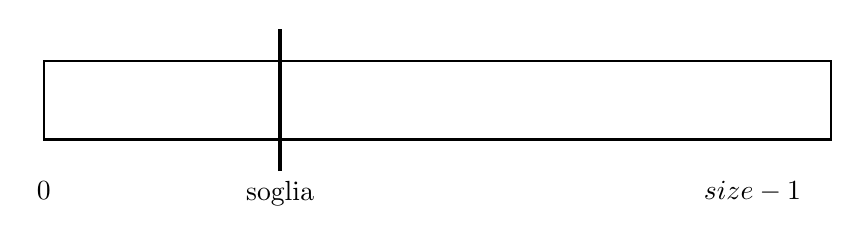
\begin{tikzpicture}
        \draw[thick] (0,0) rectangle(10,1);
        \draw[thick](0,-0.4) --(0,-0.4) node [below]{$0$};
        \draw[thick](3,-0.4) --(3,-0.4) node [below]{soglia};
        \draw[thick](9,-0.4) --(9,-0.4) node [below]{$\text{size}-1$};
        \draw[very thick] (3,-0.4) -- (3,1.4);
    \end{tikzpicture}
\end{center}

Per ordinata intendiamo che gli elementi della porzione $[0, \text{soglia}]$ siano in ordine crescente e siano tutti pi\`u piccoli degli elementi che stanno nella porzione $[\text{soglia}, \text{size}-1]$, in cui gli elementi sono distribuiti in modo arbitrario. Inoltre, gli elementi in questa seconda porzione sono tutti maggiori o uguali agli elementi che stanno in $[0, \text{soglia}-1]$.

Potenzialmente ci troveremo nel caso in cui il vettore sia disordinato e quindi avremo la soglia uguale a zero. Questo ci fa leggere la condizione come la porzione che va da $0$ a $-1$, ovvero la porzione vuota, che consideriamo ordinata. La porzione $[0,\text{size}-1]$ \`e quindi disordinata, cio\`e l'intero vettore.

Pertanto, quando analizziamo il vettore per la prima volta, ci troviamo in questa situazione nella maggior parte dei casi. Quando invece il vettore \`e completamente ordinato, la soglia varr\`a \textit{size}, poich\'e la parte tra $0$ e $\text{size}-1$ sar\`a ordinata, e quella tra \textit{size} e $\text{size}-1$ sar\`a l'intervallo vuoto (visto che l'estremo superiore \`e minore dell'estremo inferiore).

Ad ogni iterazione del ciclo dovr\`o spingere la soglia verso destra.

\begin{center}
    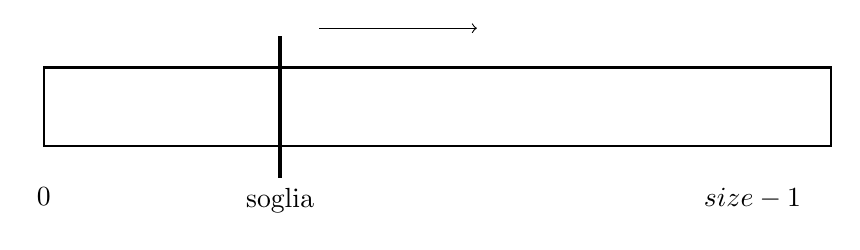
\begin{tikzpicture}
        \draw[thick] (0,0) rectangle(10,1);
        \draw[thick](0,-0.4) --(0,-0.4) node [below]{$0$};
        \draw[thick](3,-0.4) --(3,-0.4) node [below]{soglia};
        \draw[thick](9,-0.4) --(9,-0.4) node [below]{$\text{size}-1$};
        \draw[very thick] (3,-0.4) -- (3,1.4);
        \draw[->] (3.5,1.5) -- (5.5,1.5);
    \end{tikzpicture}
\end{center}

Devo prendere l'elemento pi\`u piccolo che si trova a destra; devo portarlo nella posizione successiva alla soglia e, a questo punto, la soglia viene spostata a destra, poich\'e ho rispettato la regola: ho pescato sicuramente l'elemento che \`e maggiore o uguale a quelli nella porzione $\left[0, \text{soglia}-1\right]$ e l'ho posizionato subito dopo.

\begin{center}
    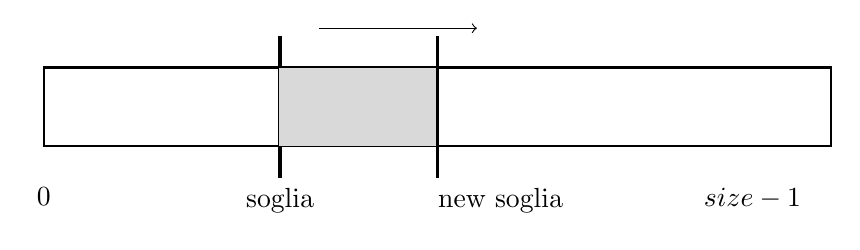
\begin{tikzpicture}
        \draw[thick] (0,0) rectangle(10,1);
        \draw[thick](0,-0.4) --(0,-0.4) node [below]{$0$};
        \draw[thick](3,-0.4) --(3,-0.4) node [below]{soglia};
        \draw[thick](9,-0.4) --(9,-0.4) node [below]{$\text{size}-1$};
        \draw[very thick] (3,-0.4) -- (3,1.4);
        \fill[gray!30] (2.99,0) rectangle (5,0.99);
        \draw[very thick] (5,-0.4) -- (5,1.4);
        \draw[thick](5.8,-0.4) --(5.8,-0.4) node [below]{new soglia};
        \draw[->] (3.5,1.5) -- (5.5,1.5);
    \end{tikzpicture}
\end{center}

\begin{codeexample}[Struttura base del bubble sort]
L'ordinamento viene implementato scorrendo il vettore dal fondo verso la soglia,
confrontando gli elementi a due a due e scambiandoli se necessario.

\begin{codebox}
\begin{lstlisting}[language=C++]
void bubble(vector<int> &v){
    for (int soglia = 0; soglia < v.size(); soglia++) {
        // La soglia deve prendere l'elemento
        // minore del range [soglia, size-1]
        // e metterlo in posizione soglia
    }
}
\end{lstlisting}
\end{codebox}
\end{codeexample}

L'ordinamento avviene se prendo il vettore e lo scorro nella direzione opposta rispetto a come scorre la soglia: dal fondo verso l'inizio. Posso considerare gli elementi a due a due: il penultimo con l'ultimo, e se l'ultimo \`e pi\`u piccolo, li scambio. Altrimenti, se sono gi\`a ordinati, non faccio nulla. Poi confronto il terzultimo con il penultimo, e cos\`i via.

Cosa succede quando arrivo all'elemento pi\`u piccolo del range soglia--size-1? L'elemento pi\`u piccolo verr\`a progressivamente spostato verso sinistra.

\begin{esempio}[Passata del bubble sort su un vettore]
Immaginiamo che la porzione che stiamo analizzando sia questa:
\begin{center}
    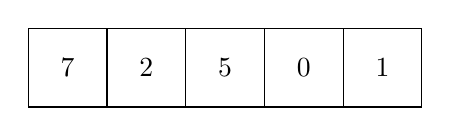
\begin{tikzpicture}
        \foreach \i/\val in {0/7,1/2,2/5,3/0,4/1} {
            \draw (\i,0) rectangle ++(1,1);
            \node at (\i+0.5,0.5) {\val};
        }
    \end{tikzpicture}
\end{center}

Comincio ad analizzare l'1 con lo 0:
\begin{itemize}
    \item Confronto l'1 con lo 0: sono disordinati.
    \begin{center}
        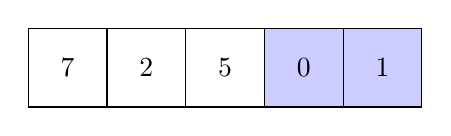
\begin{tikzpicture}
            \foreach \i/\val in {0/7,1/2,2/5,3/0,4/1} {
                \ifnum\i=3 \fill[blue!20] (\i,0) rectangle ++(1,1); \fi
                \ifnum\i=4 \fill[blue!20] (\i,0) rectangle ++(1,1); \fi
                \draw (\i,0) rectangle ++(1,1);
                \node at (\i+0.5,0.5) {\val};
            }
        \end{tikzpicture}
    \end{center}
    \item Confronto lo 0 con il 5: scambio.
    \item Confronto lo 0 con il 2: scambio.
    \item Confronto lo 0 con il 7: scambio.
\end{itemize}

Il valore 0 viene portato in prima posizione, e ottengo il seguente vettore:
\begin{center}
    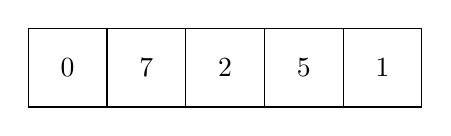
\begin{tikzpicture}
        \foreach \i/\val in {0/0,1/7,2/2,3/5,4/1} {
            \draw (\i,0) rectangle ++(1,1);
            \node at (\i+0.5,0.5) {\val};
        }
    \end{tikzpicture}
\end{center}
\end{esempio}

\begin{codeexample}[Bubble sort completo]
Implementazione completa con la funzione \texttt{swap} e il doppio ciclo.

\begin{codebox}
\begin{lstlisting}[language=C++]
void swap(int &a, int &b){
    int c = a;
    a = b;
    b = c;
}

void bubble(vector<int> &v){
    for (int soglia = 0; soglia < v.size() - 1; soglia++) {
        for (int i = v.size() - 1; i > soglia; i--) {
            if (v.at(i) < v.at(i - 1))
                swap(v.at(i), v.at(i - 1));
        }
    }
}
\end{lstlisting}
\end{codebox}

\begin{itemize}
    \item \textbf{Dove devono fermarsi questi indici?}\\
    Partendo da \lstinline{size - 1}, il primo confronto \`e tra \lstinline{v[size-1]} e \lstinline{v[size-2]}, che \`e corretto. Se mi fermassi a \textit{soglia}, l'ultimo confronto sarebbe tra \textit{soglia} e \textit{soglia-1}. Tuttavia, l'invariante del ciclo ci garantisce che l'intervallo $[0, \text{soglia}-1]$ \`e ordinato. Quindi non serve confrontare gli elementi in questa parte. Concludiamo quindi che il ciclo pu\`o fermarsi a \lstinline{i > soglia}.

    \item \textbf{\`E corretto che \lstinline{i} parta da \lstinline{size - 1}?}\\
    S\`i, perch\'e se la soglia vale \lstinline{size - 1}, il ciclo interno non si esegue (nessun confronto), ed \`e corretto: un vettore con un solo elemento \`e gi\`a ordinato. Inoltre, se il vettore ha un solo elemento, l'intero ciclo esterno far\`a solo una iterazione inutile, che possiamo evitare usando la condizione \lstinline{soglia < v.size() - 1}.

    Mettere \texttt{size - 1} come condizione di arresto implica, secondo l'invariante del ciclo, che se la parte ordinata va da \texttt{0} a \texttt{size - 2} e la parte disordinata contiene un unico elemento, allora tutto l'array pu\`o essere considerato ordinato.
\end{itemize}
\end{codeexample}

\begin{tcolorbox}[
    colback=orange!10!white,
    colframe=orange!60!black,
    boxrule=0.5pt,
    sharp corners,
    left=5mm, right=5mm,
    top=3mm, bottom=3mm,
    title=\textbf{Attenzione a \texttt{size\_t}}
]
\lstinline{v.size()} restituisce un valore di tipo \lstinline{size_t}, che \`e \textit{unsigned}. Se il vettore \`e vuoto, \lstinline{v.size() - 1} non vale $-1$, ma causa un \textit{underflow} aritmetico, producendo un valore enorme ($2^{64}-1$ su architetture a 64 bit). Il confronto \lstinline{soglia < v.size() - 1} risulterebbe quindi sempre vero, portando a un comportamento indefinito. Per evitare il problema, \`e sufficiente aggiungere un controllo iniziale \lstinline{if (v.empty()) return;} oppure effettuare un cast esplicito \lstinline{soglia < (int)v.size() - 1}.
\end{tcolorbox}

\subsection*{Ottimizzazione: terminazione anticipata}

La versione base del bubble sort esegue sempre tutti i passaggi, anche se il vettore diventa ordinato prima di completarli. Possiamo ottimizzare l'algoritmo introducendo una variabile booleana \lstinline{check} che tenga traccia di un fatto semplice: \textit{durante l'ultimo passaggio, ho effettuato almeno uno scambio?}

L'idea \`e la seguente:
\begin{itemize}
    \item All'inizio di ogni passata, assumo che il segmento sia gi\`a ordinato (\lstinline{check = false}, cio\`e ``nessuno scambio effettuato'').
    \item Se durante la passata effettuo almeno uno scambio, imposto \lstinline{check = true}.
    \item Al termine della passata, se \lstinline{check} \`e rimasto \lstinline{false}, significa che non ho fatto alcuno scambio: il vettore \`e ordinato e posso terminare.
\end{itemize}

\textbf{Attenzione:} \`e fondamentale che l'assegnamento \lstinline{check = true} si trovi \textbf{dentro} il blocco \lstinline{if}. Se lo si mette fuori dall'\lstinline{if}, la variabile viene modificata a ogni iterazione indipendentemente dallo scambio, e l'ottimizzazione non funziona.

Poich\'e la variabile \lstinline{check} viene modificata nel corpo del ciclo e usata nella condizione di arresto, la scelta stilisticamente pi\`u corretta \`e usare un ciclo \lstinline{while} per il ciclo esterno:

\begin{codeexample}[Bubble sort ottimizzato con terminazione anticipata]
Uso di un ciclo \texttt{while} e della variabile \texttt{check} per terminare
anticipatamente quando il vettore \`e gi\`a ordinato.

\begin{codebox}
\begin{lstlisting}[language=C++]
void bubble(vector<int> &v) {
    if (v.empty()) return;

    bool check = true;
    int soglia = 0;

    while (soglia < (int)v.size() - 1 && check) {
        check = false;
        for (int i = v.size() - 1; i > soglia; i--) {
            if (v[i] < v[i - 1]) {
                swap(v[i], v[i - 1]);
                check = true;  // scambio avvenuto!
            }
        }
        soglia++;
    }
}
\end{lstlisting}
\end{codebox}
\end{codeexample}

\subsection*{Stabilit\`a}

Il bubble sort \`e un algoritmo \textbf{stabile}: se due elementi hanno lo stesso valore, il loro ordine relativo nel vettore originale viene preservato. Questo accade perch\'e lo scambio avviene solo quando \lstinline{v[i] < v[i-1]} (con disuguaglianza stretta): due elementi uguali non vengono mai scambiati tra loro.

\subsection*{Ordinamento in-place}

Il bubble sort ordina il vettore \textbf{in-place}, cio\`e senza richiedere memoria aggiuntiva proporzionale alla dimensione dell'input. L'unica memoria extra utilizzata \`e quella per le variabili ausiliarie (\lstinline{soglia}, \lstinline{i}, \lstinline{check} e la variabile temporanea dello \lstinline{swap}), quindi lo spazio aggiuntivo \`e $O(1)$.












\subsection{Il codice completo}
\section{String}
\inlinecode{std::string} \`e una classe della libreria standard che incapsula
una sequenza mutabile di caratteri, con molte istruzioni e operazioni disponibili.
Dal punto di vista strutturale \`e molto simile a un \inlinecode{vector<char>}.

\subsection{Differenze rispetto a \texttt{char*}}

A differenza delle C-string (\inlinecode{char*}), \inlinecode{std::string}
offre funzionalit\`a pi\`u ricche e sicure:

\begin{itemize}
    \item \textbf{Gestione automatica della memoria}: la stringa si ridimensiona
          automaticamente quando si aggiungono o rimuovono caratteri,
          senza bisogno di allocare o deallocare memoria manualmente.

    \item \textbf{Lunghezza in tempo costante}: \inlinecode{s.size()}
          restituisce il numero di caratteri in tempo $O(1)$, poich\'e
          la lunghezza \`e mantenuta come campo interno dell'oggetto.
\end{itemize}

\subsection{Input e output}

Per leggere e scrivere stringhe si utilizzano i flussi standard:
\inlinecode{cin} per l'input e \inlinecode{cout} per l'output.

\subsection{Operazioni fondamentali}

\subsubsection{Creazione}

\begin{itemize}
    \item \inlinecode{string s;} --- crea una stringa vuota.
    \item \inlinecode{string s = "ciao";} --- inizializza la stringa con il letterale \inlinecode{"ciao"}.
\end{itemize}

\subsubsection{Assegnamento}

\begin{itemize}
    \item \inlinecode{s = "hello";} --- sostituisce l'intero contenuto di \inlinecode{s} con \inlinecode{"hello"}.
    \item \inlinecode{s = s1;} --- copia il contenuto di \inlinecode{s1} in \inlinecode{s}.
\end{itemize}

\subsubsection{Lunghezza}

\inlinecode{s.size()} e \inlinecode{s.length()} sono equivalenti e restituiscono
il numero di caratteri della stringa in tempo $O(1)$.

\subsubsection{Accesso ai caratteri}

Come per il vector, \`e possibile accedere ai singoli caratteri tramite
\inlinecode{s.at(i)}, che effettua il controllo dei limiti, oppure
tramite l'operatore \inlinecode{s[i]}. Ad esempio:
\inlinecode{s.at(i) = 'z';} modifica il carattere in posizione \inlinecode{i}.

Un pattern comune \`e iterare sui caratteri con un range-for e modificarli
in place. L'esempio seguente converte tutti i caratteri minuscoli in maiuscoli:

\begin{codeexample}[Conversione minuscolo $\to$ maiuscolo]
    \begin{codebox}
        \begin{lstlisting}
for (char& c : s) {
    if (c >= 'a' && c <= 'z')
        c = c - 'a' + 'A';
}
        \end{lstlisting}
    \end{codebox}
\end{codeexample}

\subsubsection{Confronto e ordinamento}

Le stringhe supportano gli operatori di confronto standard:

\begin{itemize}
    \item \inlinecode{s1 == s2} --- vero se le due stringhe hanno la stessa
          lunghezza e gli stessi caratteri in ogni posizione.
    \item \inlinecode{s1 != s2} --- vero se almeno un carattere \`e diverso
          o le lunghezze sono diverse.
    \item \inlinecode{s1 < s2} --- confronto lessicografico: restituisce vero
          se \inlinecode{s1} precede \inlinecode{s2} nell'ordine del dizionario.
\end{itemize}

\subsection{Concatenazione e costruzione incrementale}

Per costruire una nuova stringa per concatenazione si usa l'operatore \inlinecode{+}:

\begin{itemize}
    \item \inlinecode{string s2 = s1 + s2;} --- crea una nuova stringa concatenando
          \inlinecode{s1} e \inlinecode{s2}.
\end{itemize}

Per la \textbf{concatenazione in-place} (senza creare oggetti temporanei) si usa
l'operatore \inlinecode{+=}:

\begin{itemize}
    \item \inlinecode{s1 += s2;} --- appende \inlinecode{s2} in fondo a \inlinecode{s1},
          modificandola direttamente.
    \item \inlinecode{s1 += '!';} --- aggiunge un singolo carattere in coda.
\end{itemize}

Per la \textbf{costruzione iterativa} carattere per carattere o blocco per blocco:

\begin{itemize}
    \item \inlinecode{s.push\_back('o');} --- aggiunge il carattere \inlinecode{'o'}
          in fondo alla stringa.
    \item \inlinecode{s.append("ciao");} --- appende la sottostringa
          \inlinecode{"ciao"} in fondo.
\end{itemize}

\subsection{Estrazione, ricerca e sostituzione}

\subsubsection{Operazioni di slicing con \texttt{substr}}

\begin{itemize}
    \item \inlinecode{s.substr(pos)} --- restituisce la sottostringa che va dalla
          posizione \inlinecode{pos} fino alla fine della stringa.
    \item \inlinecode{s.substr(pos, len)} --- restituisce la sottostringa di lunghezza
          \inlinecode{len} a partire dalla posizione \inlinecode{pos}.
\end{itemize}

\begin{codeexample}[Utilizzo di \lstinline{substr}]
    \begin{codebox}
        \begin{lstlisting}
string s = "ciao mondo";
string t = s.substr(5);    // "mondo"
string u = s.substr(0, 4); // "ciao"
        \end{lstlisting}
    \end{codebox}
\end{codeexample}

\subsubsection{Operazioni di ricerca con \texttt{find}}

\begin{itemize}
    \item \inlinecode{s.find("ciao")} --- restituisce l'indice della prima occorrenza
          della sottostringa \inlinecode{"ciao"} in \inlinecode{s}, oppure
          \inlinecode{string::npos} se non trovata.
    \item \inlinecode{s.find('a')} --- versione con singolo carattere.
\end{itemize}

L'esempio seguente estrae la seconda parola di una stringa cercando il primo spazio:

\begin{codeexample}[Prima parola dopo uno spazio]
    \begin{codebox}
        \begin{lstlisting}
size_t pos = s.find(' ');
if (pos != string::npos)
    string seconda = s.substr(pos + 1);
        \end{lstlisting}
    \end{codebox}
\end{codeexample}

\subsubsection{Sostituzione con \texttt{replace}}

\inlinecode{s.replace(pos, len, "nuovo\_testo")} sostituisce \inlinecode{len}
caratteri a partire dalla posizione \inlinecode{pos} con la stringa
\inlinecode{"nuovo\_testo"}.
In un'unica operazione cancella una porzione della stringa e inserisce
il testo di rimpiazzo, che pu\`o avere lunghezza diversa.

\subsubsection{Inserimento con \texttt{insert}}

\inlinecode{s.insert(pos, "xxx")} inserisce la stringa \inlinecode{"xxx"}
alla posizione \inlinecode{pos}, spostando in avanti i caratteri successivi.

\subsubsection{Cancellazione con \texttt{erase}}

\inlinecode{s.erase(pos, len)} cancella \inlinecode{len} caratteri
a partire dalla posizione \inlinecode{pos}.

L'esempio seguente mostra l'uso combinato di \inlinecode{insert}
e \inlinecode{erase} su una stringa:

\begin{codeexample}[Inserimento e cancellazione]
    \begin{codebox}
        \begin{lstlisting}
string s = "cane";
s.insert(1, "ial"); // s diventa "cialane"
s.erase(4, 3);      // s diventa "cial"
        \end{lstlisting}
    \end{codebox}
\end{codeexample}

\section{List}

\inlinecode{std::list<T>} \`e una \textbf{lista doppiamente concatenata}:
ogni nodo contiene un elemento e due puntatori, rispettivamente al nodo
precedente e al nodo successivo. A differenza del \inlinecode{vector},
gli elementi non sono contigui in memoria ma allocati separatamente
nello heap e collegati tra loro tramite i puntatori.

\subsection{Dichiarazione e dimensione}

\begin{itemize}
    \item \inlinecode{list<int> l;} --- crea una lista vuota di interi.
    \item \inlinecode{list<int> l(n);} --- crea una lista con \inlinecode{n}
          elementi inizializzati al valore di default (\inlinecode{0} per
          \inlinecode{int}).
    \item \inlinecode{l.size();} --- restituisce il numero di elementi
          presenti nella lista.
\end{itemize}

\subsection{Inserimento e rimozione in testa e in coda}

La \inlinecode{list} supporta inserimento e rimozione in tempo $O(1)$
sia in testa che in coda:

\begin{itemize}
    \item \inlinecode{l.push\_back(x);} --- aggiunge l'elemento \inlinecode{x}
          in fondo alla lista.
    \item \inlinecode{l.push\_front(x);} --- aggiunge l'elemento \inlinecode{x}
          in testa alla lista.
    \item \inlinecode{l.pop\_back();} --- rimuove l'ultimo elemento.
    \item \inlinecode{l.pop\_front();} --- rimuove il primo elemento.
\end{itemize}












\section{Problemi e pattern di programmazione }


\begin{problema}
\textit{Funzione di lettura di un vettore.}\\
Scrivere una funzione \inlinecode{leggi} che riceva un vettore di interi per riferimento,
legga da standard input il numero di elementi e li carichi uno ad uno nel vettore.
\end{problema}

\strategia{Leggere prima la dimensione $n$, ridimensionare il vettore con \inlinecode{v.resize(n)},
poi caricare i valori uno ad uno sfruttando il range-for con riferimento.}

\begin{soluzione}
Un pattern comune \`e definire una funzione \inlinecode{leggi} che riceve
un vettore per riferimento, legge da standard input il numero di elementi
e poi li carica uno ad uno nel vettore:
\begin{enumerate}
  \item Legge un intero $n$ dallo standard input, che rappresenta
  il numero di elementi del vettore.
  \item Ridimensiona il vettore con \inlinecode{v.resize(n)}.
  \item Legge gli $n$ valori uno ad uno, caricandoli direttamente
  negli elementi del vettore.
\end{enumerate}
\begin{codeexample}[Funzione \lstinline{leggi}]
  \begin{codebox}
    \begin{lstlisting}
void leggi(std::vector<int>& v) {
    int n;
    cin >> n;
    v.resize(n);
    for (int& x : v)
        cin >> x;
}
    \end{lstlisting}
  \end{codebox}
\end{codeexample}
Il ciclo range-for con \inlinecode{int\& x} dichiara \inlinecode{x}
come \textbf{reference} all'elemento corrente del vettore.
A ogni iterazione \inlinecode{x} si lega successivamente a ciascun
elemento di \inlinecode{v}: poich\`e \`e una reference,
l'istruzione \inlinecode{cin >> x} scrive direttamente
nell'elemento del vettore, modificandolo in place.
\end{soluzione}

\subsection{Pattern esistenziale: \'e presente?}

Un pattern ricorrente sui vettori \`e verificare se esiste almeno un elemento
che soddisfa una certa propriet\`a --- si parla di \textbf{propriet\`a esistenziale}.
L'idea \`e usare un flag booleano \inlinecode{found} inizializzato a \inlinecode{false},
che viene impostato a \inlinecode{true} non appena si trova un elemento che soddisfa la condizione;
il ciclo termina anticipatamente grazie alla condizione \inlinecode{\&\& !found}.

\begin{problema}
\textit{Presenza di un elemento.}\\
Data una funzione \inlinecode{presente} che riceva un vettore di interi
\inlinecode{const vector<int>\& v} e un intero \inlinecode{x},
decidere se \inlinecode{x} \`e presente nel vettore.
\end{problema}

\strategia{Usare un flag \inlinecode{found = false} e scorrere il vettore
fino a trovare l'elemento oppure fino alla fine; restituire il flag.}

\begin{soluzione}
\begin{codeexample}[Funzione \lstinline{presente}]
  \begin{codebox}
    \begin{lstlisting}
bool presente(const vector<int>& v, int x) {
    bool found = false;
    int i = 0;
    while (i < v.size() && !found) {
        if (v.at(i) == x)
            found = true;
        i++;
    }
    return found;
}
    \end{lstlisting}
  \end{codebox}
\end{codeexample}
\end{soluzione}










\pagebreak 

\subsection{Pattern universale: tutti soddisfano la propriet\`a?}

Il duale della propriet\`a esistenziale \`e la \textbf{propriet\`a universale}:
vogliamo verificare se \emph{tutti} gli elementi soddisfano una condizione.
In questo caso il flag parte a \inlinecode{true} e viene abbattuto
non appena si trova un elemento che \emph{non} soddisfa la condizione.

\begin{problema}
\textit{Tutti i pari.}\\
Data la funzione \inlinecode{tuttiPari} che riceva un vettore di interi,
decidere se tutti gli elementi sono pari.
\end{problema}

\strategia{Usare un flag \inlinecode{found = true} e scorrere il vettore;
se si incontra un elemento dispari abbattere il flag e interrompere il ciclo.}

\begin{soluzione}
\begin{codeexample}[Funzione \lstinline{tuttiPari}]
  \begin{codebox}
    \begin{lstlisting}
bool tuttiPari(const vector<int>& v) {
    bool found = true;
    int i = 0;
    while (i < v.size() && found) {
        if (v.at(i) % 2 != 0)
            found = false;
        i++;
    }
    return found;
}
    \end{lstlisting}
  \end{codebox}
\end{codeexample}
\end{soluzione}


















\begin{problema}
\textit{Implementazione del Bubble Sort.}\\
Scrivere una funzione che ordini un vettore di interi in ordine crescente usando l'algoritmo bubble sort.
\end{problema}

\strategia{Dividere il vettore in due zone: da 0 a \texttt{soglia - 1} ordinato, da \texttt{soglia} a fine disordinato. Ad ogni passata, l'elemento più piccolo della zona disordinata ``galleggia'' verso la posizione \texttt{soglia} attraverso scambi ripetuti, poi \texttt{soglia} avanza.}

\begin{soluzione}
Il bubble sort funziona facendo ``galleggiare'' gli elementi nella posizione corretta
attraverso scambi ripetuti tra elementi adiacenti.
Abbiamo un vettore diviso in due zone da una variabile \inlinecode{soglia}:
da indice 0 a \inlinecode{soglia - 1} la zona \`e ordinata, da \inlinecode{soglia}
a fine vettore la zona \`e disordinata.
All'inizio \inlinecode{soglia = 0} (niente \`e ordinato).
Ad ogni passata, l'elemento pi\`u piccolo della zona disordinata ``galleggia''
fino alla posizione \inlinecode{soglia}, e poi \inlinecode{soglia} avanza di 1.

\begin{codeexample}[Funzione \lstinline{bubble}]
  \begin{codebox}
    \begin{lstlisting}
void bubble(vector<int>& v) {
    if (v.empty()) return;          // (1)
    int soglia = 0;                 // (2)
    while (soglia < (int)v.size() - 1) {   // (3)
        for (int i = v.size() - 1; i > soglia; i--) {  // (4)
            if (v.at(i) < v.at(i - 1)) {         // (5)
                swap(v.at(i), v.at(i - 1));      // (6)
            }
        }
        soglia++;                   // (7)
    }
}
    \end{lstlisting}
  \end{codebox}
\end{codeexample}

\textbf{Analisi riga per riga:}
\begin{enumerate}
  \item \inlinecode{if (v.empty()) return;} --- Se il vettore \`e vuoto non c'\`e nulla da ordinare.
  Senza questo controllo, \inlinecode{v.size() - 1} su un vettore vuoto darebbe un numero enorme
  (perch\'e \inlinecode{size()} restituisce un \inlinecode{unsigned}, e $0 - 1$ in unsigned va in overflow).
  
  \item \inlinecode{int soglia = 0;} --- Inizializziamo la soglia a 0:
  ``nessun elemento \`e ancora nella posizione corretta''.
  Tutta la zona da 0 a \inlinecode{v.size()-1} \`e disordinata.
  
  \item \inlinecode{while (soglia < (int)v.size() - 1)} --- Il ciclo esterno continua finch\'e
  la soglia non ha raggiunto la penultima posizione.
  Perch\'e penultima e non ultima? Perch\'e se tutti gli elementi tranne l'ultimo sono al posto giusto,
  anche l'ultimo per forza lo \`e.
  Il cast \inlinecode{(int)} serve perch\'e \inlinecode{v.size()} \`e unsigned.
  
  \item \inlinecode{for (int i = v.size() - 1; i > soglia; i--)} --- Questo \`e il ciclo interno.
  Parte dall'ultimo elemento del vettore e scende verso la soglia.
  Perch\'e dal fondo? Perch\'e vogliamo far ``salire'' l'elemento pi\`u piccolo verso sinistra,
  verso la posizione soglia.
  \inlinecode{i > soglia} e non \inlinecode{i >= soglia} perch\'e nel corpo del \inlinecode{for}
  confrontiamo \inlinecode{v[i]} con \inlinecode{v[i-1]}.
  Se \inlinecode{i} fosse uguale a \inlinecode{soglia}, allora \inlinecode{i-1} sarebbe
  \inlinecode{soglia - 1}, cio\`e andremmo a toccare la zona gi\`a ordinata, che non va toccata.
  
  \item \inlinecode{if (v.at(i) < v.at(i - 1))} --- Confrontiamo l'elemento corrente con quello che lo precede.
  Se quello corrente \`e pi\`u piccolo, sono nell'ordine sbagliato (perch\'e vogliamo ordine crescente).
  
  \item \inlinecode{swap(v.at(i), v.at(i - 1));} --- Li scambiamo.
  Dopo lo scambio, l'elemento pi\`u piccolo si \`e spostato di una posizione verso sinistra.
  Questo succede ripetutamente lungo tutto il ciclo \inlinecode{for},
  quindi l'elemento pi\`u piccolo della zona disordinata ``galleggia'' fino a \inlinecode{soglia}.
  
  \item \inlinecode{soglia++;} --- La passata \`e finita.
  L'elemento pi\`u piccolo della zona disordinata \`e arrivato in posizione \inlinecode{soglia}.
  Ora quella posizione fa parte della zona ordinata, quindi avanziamo la soglia di 1.
\end{enumerate}
\end{soluzione}

\subsection{Esempio di esecuzione}

\section*{Legenda}
\begin{tikzpicture}
    \node[draw, fill=ordinato, minimum width=0.6cm, minimum height=0.6cm, rounded corners=2pt] at (0,0) {};
    \node[right] at (0.5,0) {Ordinato (sotto soglia)};
    \node[draw, fill=confronto, minimum width=0.6cm, minimum height=0.6cm, rounded corners=2pt] at (5.4,0) {};
    \node[right] at (5.8,0) {Confronto};
    \node[draw, fill=scambio, minimum width=0.6cm, minimum height=0.6cm, rounded corners=2pt] at (9,0) {};
    \node[right] at (9.5,0) {Scambio};
    \node[draw, fill=neutro, minimum width=0.6cm, minimum height=0.6cm, rounded corners=2pt] at (13,0) {};
    \node[right] at (13.5,0) {Disordinato};
\end{tikzpicture}

\bigskip
Vettore iniziale: $[5, 3, 1, 4, 2]$, \quad $\text{soglia} = 0$

%===========================================
\section*{Passata 1}
$\text{soglia} = 0$, \quad il \texttt{for} va da $i=4$ fino a $i>0$ \quad (4 confronti)

\bigskip
\textbf{Stato iniziale:}
\begin{center}
\begin{tikzpicture}
    \foreach \x/\v in {0/5, 1.2/3, 2.4/1, 3.6/4, 4.8/2} {
        \cella{\x}{neutro}; \num{\x}{\v};
    }
\end{tikzpicture}
\end{center}

$i=4$: $v[4]=2 < v[3]=4$ \checkmark $\Rightarrow$ \textbf{swap!}
\begin{center}
\begin{tikzpicture}
    \foreach \x/\v/\c in {0/5/neutro, 1.2/3/neutro, 2.4/1/neutro, 3.6/2/scambio, 4.8/4/scambio} {
        \cella{\x}{\c}; \num{\x}{\v};
    }
\end{tikzpicture}
\end{center}

$i=3$: $v[3]=2 < v[2]=1$? No $\Rightarrow$ nessuno scambio
\begin{center}
\begin{tikzpicture}
    \foreach \x/\v/\c in {0/5/neutro, 1.2/3/neutro, 2.4/1/confronto, 3.6/2/confronto, 4.8/4/neutro} {
        \cella{\x}{\c}; \num{\x}{\v};
    }
\end{tikzpicture}
\end{center}

$i=2$: $v[2]=1 < v[1]=3$ \checkmark $\Rightarrow$ \textbf{swap!}
\begin{center}
\begin{tikzpicture}
    \foreach \x/\v/\c in {0/5/neutro, 1.2/1/scambio, 2.4/3/scambio, 3.6/2/neutro, 4.8/4/neutro} {
        \cella{\x}{\c}; \num{\x}{\v};
    }
\end{tikzpicture}
\end{center}

$i=1$: $v[1]=1 < v[0]=5$ \checkmark $\Rightarrow$ \textbf{swap!}
\begin{center}
\begin{tikzpicture}
    \foreach \x/\v/\c in {0/1/scambio, 1.2/5/scambio, 2.4/3/neutro, 3.6/2/neutro, 4.8/4/neutro} {
        \cella{\x}{\c}; \num{\x}{\v};
    }
\end{tikzpicture}
\end{center}

$\text{soglia++} \Rightarrow \text{soglia} = 1$
\begin{center}
\begin{tikzpicture}
    \foreach \x/\v/\c in {0/1/ordinato, 1.2/5/neutro, 2.4/3/neutro, 3.6/2/neutro, 4.8/4/neutro} {
        \cella{\x}{\c}; \num{\x}{\v};
    }
\end{tikzpicture}
\end{center}

%===========================================
\section*{Passata 2}
$\text{soglia} = 1$, \quad il \texttt{for} va da $i=4$ fino a $i>1$ \quad (3 confronti)

\bigskip
$i=4$: $v[4]=4 < v[3]=2$? No $\Rightarrow$ nessuno scambio
\begin{center}
\begin{tikzpicture}
    \foreach \x/\v/\c in {0/1/ordinato, 1.2/5/neutro, 2.4/3/neutro, 3.6/2/confronto, 4.8/4/confronto} {
        \cella{\x}{\c}; \num{\x}{\v};
    }
\end{tikzpicture}
\end{center}

$i=3$: $v[3]=2 < v[2]=3$ \checkmark $\Rightarrow$ \textbf{swap!}
\begin{center}
\begin{tikzpicture}
    \foreach \x/\v/\c in {0/1/ordinato, 1.2/5/neutro, 2.4/2/scambio, 3.6/3/scambio, 4.8/4/neutro} {
        \cella{\x}{\c}; \num{\x}{\v};
    }
\end{tikzpicture}
\end{center}

$i=2$: $v[2]=2 < v[1]=5$ \checkmark $\Rightarrow$ \textbf{swap!}
\begin{center}
\begin{tikzpicture}
    \foreach \x/\v/\c in {0/1/ordinato, 1.2/2/scambio, 2.4/5/scambio, 3.6/3/neutro, 4.8/4/neutro} {
        \cella{\x}{\c}; \num{\x}{\v};
    }
\end{tikzpicture}
\end{center}

$\text{soglia++} \Rightarrow \text{soglia} = 2$
\begin{center}
\begin{tikzpicture}
    \foreach \x/\v/\c in {0/1/ordinato, 1.2/2/ordinato, 2.4/5/neutro, 3.6/3/neutro, 4.8/4/neutro} {
        \cella{\x}{\c}; \num{\x}{\v};
    }
\end{tikzpicture}
\end{center}

%===========================================
\section*{Passata 3}
$\text{soglia} = 2$, \quad il \texttt{for} va da $i=4$ fino a $i>2$ \quad (2 confronti)

\bigskip
$i=4$: $v[4]=4 < v[3]=3$? No $\Rightarrow$ nessuno scambio
\begin{center}
\begin{tikzpicture}
    \foreach \x/\v/\c in {0/1/ordinato, 1.2/2/ordinato, 2.4/5/neutro, 3.6/3/confronto, 4.8/4/confronto} {
        \cella{\x}{\c}; \num{\x}{\v};
    }
\end{tikzpicture}
\end{center}

$i=3$: $v[3]=3 < v[2]=5$ \checkmark $\Rightarrow$ \textbf{swap!}
\begin{center}
\begin{tikzpicture}
    \foreach \x/\v/\c in {0/1/ordinato, 1.2/2/ordinato, 2.4/3/scambio, 3.6/5/scambio, 4.8/4/neutro} {
        \cella{\x}{\c}; \num{\x}{\v};
    }
\end{tikzpicture}
\end{center}

$\text{soglia++} \Rightarrow \text{soglia} = 3$
\begin{center}
\begin{tikzpicture}
    \foreach \x/\v/\c in {0/1/ordinato, 1.2/2/ordinato, 2.4/3/ordinato, 3.6/5/neutro, 4.8/4/neutro} {
        \cella{\x}{\c}; \num{\x}{\v};
    }
\end{tikzpicture}
\end{center}

%===========================================
\section*{Passata 4}
$\text{soglia} = 3$, \quad il \texttt{for} va da $i=4$ fino a $i>3$ \quad (1 confronto)

\bigskip
$i=4$: $v[4]=4 < v[3]=5$ \checkmark $\Rightarrow$ \textbf{swap!}
\begin{center}
\begin{tikzpicture}
    \foreach \x/\v/\c in {0/1/ordinato, 1.2/2/ordinato, 2.4/3/ordinato, 3.6/4/scambio, 4.8/5/scambio} {
        \cella{\x}{\c}; \num{\x}{\v};
    }
\end{tikzpicture}
\end{center}

$\text{soglia++} \Rightarrow \text{soglia} = 4$
\begin{center}
\begin{tikzpicture}
    \foreach \x/\v/\c in {0/1/ordinato, 1.2/2/ordinato, 2.4/3/ordinato, 3.6/4/ordinato, 4.8/5/ordinato} {
        \cella{\x}{\c}; \num{\x}{\v};
    }
\end{tikzpicture}
\end{center}

%===========================================
\section*{Terminazione}

$\text{soglia} = 4 < v.\text{size}() - 1 = 4$ ? \quad \textbf{No} $\Rightarrow$ il \texttt{while} termina.

\bigskip
\textbf{Risultato finale:} $[1, 2, 3, 4, 5]$ \checkmark



\subsection{Ottimizzazione: terminazione anticipata}

\begin{problema}
\textit{Bubble Sort con early termination.}\\
Modificare la funzione bubble sort per terminare anticipatamente se il vettore è già ordinato.
\end{problema}

\strategia{Usare un flag booleano \texttt{check} che viene resettato a \texttt{false} all'inizio di ogni passata. Se durante la passata avviene almeno uno scambio, \texttt{check} viene impostato a \texttt{true}. Se alla fine di una passata \texttt{check} è ancora \texttt{false}, significa che non ci sono stati scambi e il vettore è già ordinato, quindi possiamo terminare.}

\begin{soluzione}
\begin{codeexample}[Bubble sort con early termination]
  \begin{codebox}
    \begin{lstlisting}
void bubble(vector<int>& v) {
    if (v.empty()) return;

    bool check = true;
    int soglia = 0;

    while (soglia < (int)v.size() - 1 && check) {
        check = false;
        for (int i = v.size() - 1; i > soglia; i--) {
            if (v[i] < v[i - 1]) {
                swap(v[i], v[i - 1]);
                check = true;
            }
        }
        soglia++;
    }
}
    \end{lstlisting}
  \end{codebox}
\end{codeexample}
\end{soluzione}

\subsection{Esempio di early termination}

\section*{Legenda}
\begin{tikzpicture}
    \node[draw, fill=confronto, minimum width=0.6cm, minimum height=0.6cm, rounded corners=2pt] at (0,0) {};
    \node[right] at (0.5,0) {Confronto};
    \node[draw, fill=scambio, minimum width=0.6cm, minimum height=0.6cm, rounded corners=2pt] at (4,0) {};
    \node[right] at (4.5,0) {Scambio};
    \node[draw, fill=neutro, minimum width=0.6cm, minimum height=0.6cm, rounded corners=2pt] at (8,0) {};
    \node[right] at (8.5,0) {Non toccato};
    \node[draw, fill=ordinato, minimum width=0.6cm, minimum height=0.6cm, rounded corners=2pt] at (12,0) {};
    \node[right] at (12.5,0) {Tutto ordinato};
\end{tikzpicture}

\bigskip
\textbf{Nota:} in questo esercizio \textbf{non c'\`e la soglia}. Il \texttt{for} scorre sempre tutto il vettore. L'unica ottimizzazione \`e il flag \texttt{check}: se una passata intera non produce scambi, il vettore \`e gi\`a ordinato e ci fermiamo.

\bigskip
Vettore iniziale: $[1, 3, 2, 4, 5]$ (quasi ordinato, solo 3 e 2 invertiti)

%===========================================
\section*{Passata 1}
\texttt{check} viene resettato a \texttt{false} \quad $\Rightarrow$ \quad il \texttt{for} va da $i=4$ fino a $i>0$ \quad (4 confronti)

\bigskip
\textbf{Stato iniziale:}
\begin{center}
\begin{tikzpicture}
    \foreach \x/\v in {0/1, 1.2/3, 2.4/2, 3.6/4, 4.8/5} {
        \cella{\x}{neutro}; \num{\x}{\v};
    }
\end{tikzpicture}
\end{center}

$i=4$: $v[4]=5 < v[3]=4$? No $\Rightarrow$ nessuno scambio
\begin{center}
\begin{tikzpicture}
    \foreach \x/\v/\c in {0/1/neutro, 1.2/3/neutro, 2.4/2/neutro, 3.6/4/confronto, 4.8/5/confronto} {
        \cella{\x}{\c}; \num{\x}{\v};
    }
\end{tikzpicture}
\end{center}

$i=3$: $v[3]=4 < v[2]=2$? No $\Rightarrow$ nessuno scambio
\begin{center}
\begin{tikzpicture}
    \foreach \x/\v/\c in {0/1/neutro, 1.2/3/neutro, 2.4/2/confronto, 3.6/4/confronto, 4.8/5/neutro} {
        \cella{\x}{\c}; \num{\x}{\v};
    }
\end{tikzpicture}
\end{center}

$i=2$: $v[2]=2 < v[1]=3$ \checkmark $\Rightarrow$ \textbf{swap!} \quad \texttt{check = true}
\begin{center}
\begin{tikzpicture}
    \foreach \x/\v/\c in {0/1/neutro, 1.2/2/scambio, 2.4/3/scambio, 3.6/4/neutro, 4.8/5/neutro} {
        \cella{\x}{\c}; \num{\x}{\v};
    }
\end{tikzpicture}
\end{center}

$i=1$: $v[1]=2 < v[0]=1$? No $\Rightarrow$ nessuno scambio
\begin{center}
\begin{tikzpicture}
    \foreach \x/\v/\c in {0/1/confronto, 1.2/2/confronto, 2.4/3/neutro, 3.6/4/neutro, 4.8/5/neutro} {
        \cella{\x}{\c}; \num{\x}{\v};
    }
\end{tikzpicture}
\end{center}

\textbf{Fine passata 1:} \texttt{check = true} $\Rightarrow$ \`e avvenuto almeno uno scambio $\Rightarrow$ \textbf{si continua}

\begin{center}
\begin{tikzpicture}
    \foreach \x/\v in {0/1, 1.2/2, 2.4/3, 3.6/4, 4.8/5} {
        \cella{\x}{neutro}; \num{\x}{\v};
    }
\end{tikzpicture}
\end{center}

%===========================================
\section*{Passata 2}
\texttt{check} viene resettato a \texttt{false} \quad $\Rightarrow$ \quad il \texttt{for} va da $i=4$ fino a $i>0$ \quad (4 confronti)

\bigskip
$i=4$: $v[4]=5 < v[3]=4$? No $\Rightarrow$ nessuno scambio
\begin{center}
\begin{tikzpicture}
    \foreach \x/\v/\c in {0/1/neutro, 1.2/2/neutro, 2.4/3/neutro, 3.6/4/confronto, 4.8/5/confronto} {
        \cella{\x}{\c}; \num{\x}{\v};
    }
\end{tikzpicture}
\end{center}

$i=3$: $v[3]=4 < v[2]=3$? No $\Rightarrow$ nessuno scambio
\begin{center}
\begin{tikzpicture}
    \foreach \x/\v/\c in {0/1/neutro, 1.2/2/neutro, 2.4/3/confronto, 3.6/4/confronto, 4.8/5/neutro} {
        \cella{\x}{\c}; \num{\x}{\v};
    }
\end{tikzpicture}
\end{center}

$i=2$: $v[2]=3 < v[1]=2$? No $\Rightarrow$ nessuno scambio
\begin{center}
\begin{tikzpicture}
    \foreach \x/\v/\c in {0/1/neutro, 1.2/2/confronto, 2.4/3/confronto, 3.6/4/neutro, 4.8/5/neutro} {
        \cella{\x}{\c}; \num{\x}{\v};
    }
\end{tikzpicture}
\end{center}

$i=1$: $v[1]=2 < v[0]=1$? No $\Rightarrow$ nessuno scambio
\begin{center}
\begin{tikzpicture}
    \foreach \x/\v/\c in {0/1/confronto, 1.2/2/confronto, 2.4/3/neutro, 3.6/4/neutro, 4.8/5/neutro} {
        \cella{\x}{\c}; \num{\x}{\v};
    }
\end{tikzpicture}
\end{center}

\textbf{Fine passata 2:} \texttt{check = false} $\Rightarrow$ \textbf{nessuno scambio in tutta la passata!}

\bigskip
Questo significa che per ogni $i$: $v[i-1] \leq v[i]$, cio\`e ogni elemento \`e minore o uguale del successivo.

Quindi il vettore \`e \textbf{gi\`a ordinato} e possiamo \textbf{terminare}.

\begin{center}
\begin{tikzpicture}
    \foreach \x/\v in {0/1, 1.2/2, 2.4/3, 3.6/4, 4.8/5} {
        \cella{\x}{ordinato}; \num{\x}{\v};
    }
\end{tikzpicture}
\end{center}

%===========================================
\section*{Terminazione}

Il \texttt{while} controlla \texttt{check}:

$$\texttt{check} = \texttt{false} \quad \Rightarrow \quad \text{il \texttt{while} termina}$$

\textbf{Risultato finale:} $[1, 2, 3, 4, 5]$ \checkmark

%===========================================
\section*{Confronto con il Bubble Sort senza early termination}

\begin{center}
\begin{tabular}{|l|c|c|}
\hline
& \textbf{Senza early termination} & \textbf{Con early termination} \\
\hline
Passate eseguite & $n - 1 = 4$ & $2$ \\
\hline
Confronti totali & $\dfrac{n(n-1)}{2} = 10$ & $4 + 4 = 8$ \\
\hline
\end{tabular}
\end{center}

\bigskip
In questo esempio abbiamo risparmiato 2 passate e 2 confronti. Il vantaggio diventa enorme con vettori grandi e quasi ordinati.

%===========================================
\section*{Caso estremo: vettore gi\`a ordinato}

Vettore: $[1, 2, 3, 4, 5]$

\bigskip
\textbf{Passata 1:} \texttt{check} resettato a \texttt{false}

\begin{center}
\begin{tabular}{ll}
$i=4$: $v[4]=5 < v[3]=4$? & No \\
$i=3$: $v[3]=4 < v[2]=3$? & No \\
$i=2$: $v[2]=3 < v[1]=2$? & No \\
$i=1$: $v[1]=2 < v[0]=1$? & No \\
\end{tabular}
\end{center}

\texttt{check} \`e ancora \texttt{false} $\Rightarrow$ \textbf{esco dopo una sola passata!}

$$\text{Costo:} \quad n - 1 = 4 \text{ confronti} \quad \Rightarrow \quad O(n)$$

Senza early termination avremmo fatto $\dfrac{n(n-1)}{2} = 10$ confronti $\Rightarrow O(n^2)$.

%===========================================
\section*{Riepilogo complessit\`a}

\begin{align*}
    \textbf{Caso migliore} \text{ (vettore gi\`a ordinato):} &\quad O(n) \\
    \textbf{Caso medio:} &\quad O(n^2) \\
    \textbf{Caso peggiore} \text{ (vettore ordinato al contrario):} &\quad O(n^2) \\
    \textbf{Spazio:} &\quad O(1) \text{ (in-place)}
\end{align*}
